\documentclass[a4paper,10pt,twoside]{report}
\usepackage[utf8]{inputenc}
\usepackage[T1]{fontenc} 
\usepackage{ucs}
\usepackage[english]{babel}
\usepackage{float}
\usepackage{lscape}
\usepackage[final]{pdfpages}
\usepackage{geometry}
\geometry{hmargin=2.0cm,vmargin=2.0cm}
\usepackage{setspace}
\onehalfspacing

\renewcommand{\thesection}{\arabic{section}}

\title{Pan-genomics in plants}
\author{Cécile Monat - Francois Sabot}

\begin{document}
\maketitle
% * <cmonat26@gmail.com> 2018-05-24T15:06:18.412Z:
%
% ^.
\section{Introduction}
Understanding diversity between individuals is a key point to understand their phenotypic variations, as well as mechanisms allowing environmental adaptation \cite{Hirsch2014, Guimaraes2015}. Estimation of diversity is based on the currently available methods and technologies at a time. Carl Von Linné or Georges-Louis de Buffon classified animals and plants based on visual phenotypic observations. Nowadays biologists deal with molecular data, and diversity estimation is based on genetics and genomics dataset. 

Nowadays, diversity studies are mainly performed using SNP (Single Nucleotide Polymorphism) \cite{Springer2009, Hirsch2014} detected through NGS (Next Generation Sequencing). The allelic diversity in coding and non-coding sequences is generally though to be the main cause of phenotypic variations. Until recently, it was generally admitted that individuals from the same species have a similar genetic content \cite{Swanson-Wagner2010} and differ only by few SNP. However, since the rise of NGS and of massive sequencing, it appeared that structural variation (SV) in the form of small insertion deletions (Indel), large up to tens of kb, but also chromosomal rearrangements, are much more important than expected \ref{PAVcaption}. These variations might be due to CNV (Copy Number Variation) of the same sequence, or even missing sequences in some individuals (PAV, Presence/Absence Variations) \cite{DaSilva2013,Montenegro2017}. Those different levels of diversity (SNP, SV, CNV and PAV) add a challenge in the representation of the genome of a species. It is now clear that we need more assembled individual genomes (and more variation informations) to capture the whole diversity of a given species. Indeed, a single reference genome is not enough anymore to define the variability in a species \cite{Gan2011,Li2014b,Hirsch2014,Schatz2014}.\\

\begin{figure}[ht]
\centering

 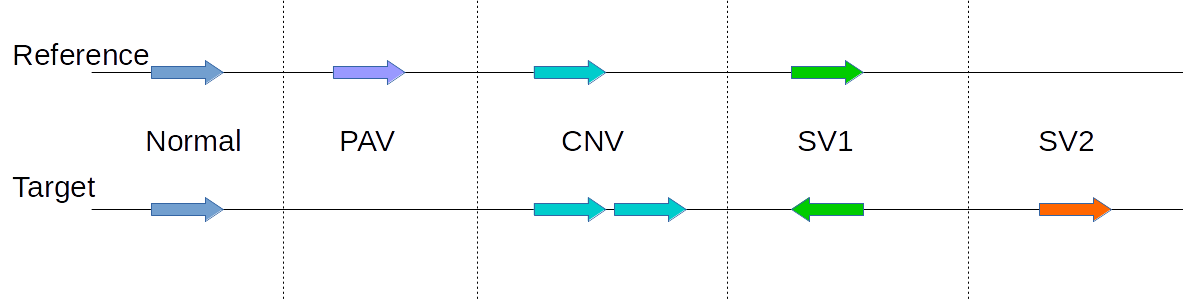
\includegraphics[scale=1]{PAVcnvSV.png}
% * <cmonat26@gmail.com> 2018-05-15T13:45:48.053Z:
% 
% Sur cette figue, SV2 est exactement equivalent a PAV.
% Pour l'insertion, il vaudrait mieux représenter un flèche existante chez les deux séquences, mais qu'elle soit par ex. plus longue chez un des deux pour représenter l'insertion/deletion de sequence chez l'un/l'autre.
% En SV, il manque les translocations. 
% Je propose que plutôt que d'utiliser une couleur différente pour chaque type de variation, on se serve de couleur pour différencier les SV qui change la quantité de séquence (couleur1 - PAV, CNV) vs les SV qui conserve (couleur2 - inversions, translocations). Tu vois l'idée ?
% Et plutôt que Reference et Target, je mettrai Query et Subject (pour aller dans le sens, qu'un seul génome de ref, ça pue ^^)
% 
% ^.
 \caption{Schematic representation of PAV (Presence/Absence Variation), CNV (Copy Number Variation) and SV (Structural Variations) between a reference sequence and a target genome. Each colored arrow represents a genomic segment. SV1: invertion. SV2: insertion.}
 \label{PAVcaption}
\end{figure}

\section{Pan-genome concept}

The access to DNA sequences, \textit{i.e.} to the whole genetic information, has not evolved at the same pace for the different phylum, mainly because of the genome size of the organisms. For instance, microorganisms (ex: \emph{Saccharomyces cerevisiae} 13 Mb) and bacteria (ex: \emph{Escherichia coli} 4.6 Mb) are mostly small genomes, easy to sequence and assemble. In  opposite, few plant genomes are available so far due to their size (Gb sized) and higher complexity (polyploidy, high percentage of repetitive sequences, partial and whole genome duplication,...). Thus, the true first pan-genomic studies were performed on small bacterial genomes \cite{Tettelin2005,Tettelin2008} before plants. 

The concept was first introduced in 2005 by Tettelin et al as follows: the pan-genome consists of a "core genome containing genes present in all strains and a dispensable genome composed of genes absent from one or more strains and genes that are unique to each strain" \cite{Tettelin2005}(Figure~\ref{pangenome}). This definition has been since re-used many times \cite{Tettelin2008,Liang2012,Lukjancenko2012,Mann2013,Lukjancenko2013,Kahlke2013,Soares2013} and extended to transcripts, proteins, pseudogenes as well as to TEs (Transposable Elements) \cite{Lukjancenko2013,Nguyen2014,Hirsch2014}. A pan-genomic analysis allows to characterize the folder of genes/sequences available within a given group, as well as to estimate the missing genomic quantity (\textit{i.e.} the number of new individuals to be sequenced) needed to complete it \cite{Tettelin2008}. We may, by such means, better understand the ecological adaptations and have a more complete view on how genetic variation is important for adaptation and survival of a given group \cite{Hansen2012}. Such studies are performed on a set of organisms/individuals supposed to be representative of a family, a genera or more generally a species. Pan-genomic analyses provide a large array of phylogenomics information at different levels, from general implications of the group to individual-specific genetic information \cite{Kahlke2013,Soares2013}.

\begin{figure}[h]
\centering
 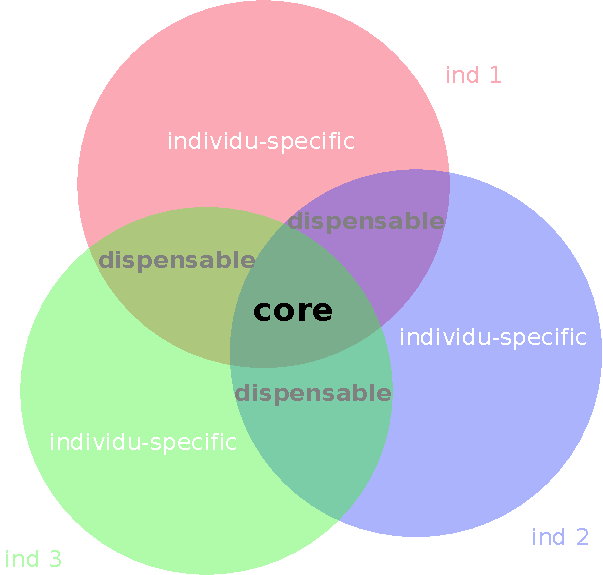
\includegraphics[scale=1]{panG.pdf}
 \caption[Pan-genome of three individuals]{Pan-genome of three individuals. Each individual is represented by a different color. Intersection between the three circles represents the core genome, intersections between two the dispensable genome, and parts without intersection the individual-specific genome. Adapted from Tettelin et al \cite{Tettelin2005}}
 \label{pangenome}
\end{figure}

\subsection{Core-genome}
The core-genome is made of genes/sequences present in all individuals of the studied group \cite{Lukjancenko2012,Lukjancenko2013,Soares2013}. In bacteria, those genes are conserved and seem to be, for most, important genes for basic biological processes \cite{Tettelin2005,Soares2013}, and have been qualified as essential \cite{Kahlke2013}. However, the more individuals are added to the study, the less core-genes are found  \cite{Tettelin2005,Lukjancenko2012}, and the core-genome is generally over-estimated.
In addition, Collins et al \cite{Collins2012} shown that genes considered as essential -qualified as it because of their function which seems to be essential for the survival of the individual- might be absent from the core-genome.  So the level of definition of essential is critical in the way of interpretation of core-genome. In this regard, core-genome would be composed of putatively essential (functionally essentials) genes but also of genes evolving slowly enough to be present in each genome (pan-genomically defined as essential), not required for their host survival.

\subsection{Dispensable-genome}
Dispensable genes are genes found in at least two individuals among those studied, but not in all \cite{Tettelin2005,Liang2012}. These genes mostly belong to secondary biological processes, and are associated with adaptation, resistance to biotic and abiotic stresses or, for microorganisms, new host colonization \cite{Tettelin2008,Mann2013,Hirsch2014}. In rice, Schatz et al \cite{Schatz2014} shown that some are related to disease resistance genes, even if the frequency of those type of genes is much higher for the genes of the individual-specific-genome (see below).

Those genes are supposed to be the main contributors of the variability of a species \cite{Kahlke2013}. Their origin is supposed to be distinct regarding the phylum: in bacteria, they probably originate from horizontal transfers \cite{Medini2005}, while in eukaryots they may be related to genes lost, segmental of whole-genome duplications, neogenesis, or even related to TEs activity \cite{Hirsch2014}. 

\subsection{Individual-specific-genome}
\label{individual}
Genes belonging to a single individual are regrouped under the term of individual-specific-genome  \cite{Tettelin2005,Lukjancenko2013,Soares2013}. In microorganisms and bacteria, they are mostly related to phages, horizontal transfers or TEs \cite{Kahlke2013}. In rice, Schatz et al \cite{Schatz2014} shown that most of these sequences are repetitive sequences, some being genes related. They also shown that the distribution of these unique regions is not precisely located but well distributed among the genome. Different studies shown that new genes, or genes recently evolved, have generally smaller CDS (Coding DNA Sequence) compared to older/strictly conserved genes \cite{Cai2010, Capra2010, Lipman2002}, such as those of the individual-specific-genome, which suggest they might be new or recently evolved \cite{Schatz2014}.

\subsection{Pan-genome}
The size of the pan-genome depends on the number of genes found in the sampled individuals. Pan-genome might be open or closed depending on the size of it (\texttt{Figure~\ref{openOrClosed}}): if the size increases at each new added individual then, it is considered as open \cite{Mann2013}. On the opposite, if after a certain number of individual the size reaches a plateau, then it is a closed pan-genome. As the pan-genome is changing depending on how many individuals are included in the study, it is important to know, for a given population, from how many studied genomes is the diversity almost completely represented \cite{Tatusov1997,Tettelin2005,Hogg2007,Tettelin2008}.

Bacterial species with a closed pan-genome seems to be living in isolated niches or have a low capacity to acquire new genes \cite{Koonin2005}


\begin{figure}[h]
\centering
 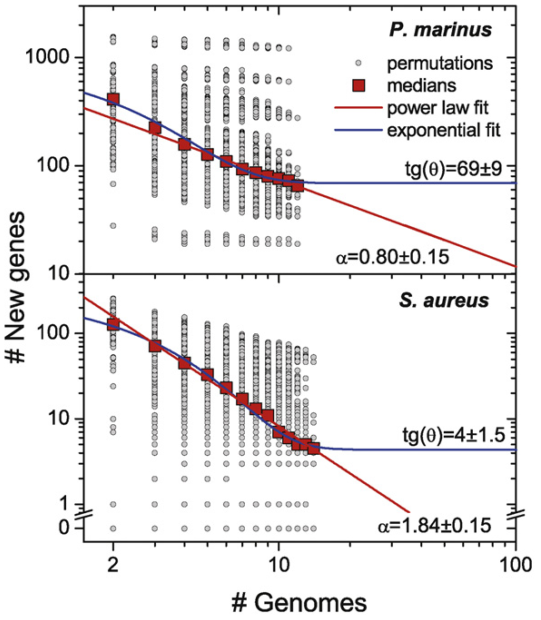
\includegraphics[scale=0.5]{Tettelin2088_OpenAndClosedPanGenome.png}
 \caption[Open or closed pan-genome]{Open or closed pan-genome. Exhibitor $\alpha$ determine if pan-genome is open ($\alpha$ $\leq$ 1) or closed ($\alpha$ $>$ 1).
From Tettelin et al \cite{Tettelin2008}}
 \label{openOrClosed}
\end{figure}

\subsection{Ten years of pan-genomics}
Since the beginning of pan-genomics \cite{Tettelin2005}, many projects have been performed on different organisms (bacteria, \textit{archaea}, animals, plants, virus and recently fungi) with a high variation in the range of studied genomes (from 2 individuals to 14,129, \cite{Lu2015}) and how many species are used to (between 1 and 3, \cite{Darling2010, Gordienko2013, Boussaha2015, Ghatak2016}). Many different methods have been used to be adapted to each data set (see \cite{Vernikos2015} for more details). \\

\section{Pan-genome structure depends on the population one}
Pan-genome size is supposed to vary based on the size of the genomes studied \cite{Tatusov1997, Hogg2007, Hirsch2014}: the bigger the genome is, the bigger the pan-genome might be \cite{Tatusov1997,Hogg2007,Hirsch2014}. Depending to the species studied (internal variability), the number of individual required to be representative of the variability of the species is variable. To perform a pan-genomic study, the choice of the individuals and how many are included in the study is then extremely important \cite{Tatusov1997,Tettelin2005,Hogg2007,Tettelin2008}.\\

Some studies shown that analyzing many genomes of the same species allowed to discover more intra-specific diversity than expected \cite{Tettelin2008}. Working on many individuals from the same species lead to identify a diversity which might be not visible if we only look inter-species variability \cite{Lukjancenko2012}. In addition, two genomes are not only similar to each other because of the genes they share, but also if they missed the same ones \cite{Snipen2010}.\\

%To represent a species, in most of the case, a single genome is assembled and annotated using high-quality data. This genome is then considered as the reference genome for the considered species, and the representation of a species is then seen through this single individual. This is a very limiting vision of what is a species, as this individual cannot contain the whole variability of its species \cite{Nguyen2014}. So, having one reference genome to study the diversity of a species is not the best way to do analyze the potentially available diversity of the species.

%A pan-genomic analyze because it includes many individual, might be a better representation of the diversity of one species. Especially because the quantity of individual will always be a better median to represent the observed diversity than one single individual \cite{Nguyen2014}. Pan-genome is, therefore, a good representation of the whole genes presents in the studied group of individuals ( a group which can be assimilated to a population or a species).\\

\subsection{Pan-genomic in plants}
In plants, there have been at least 13 pan-genomics studies (\texttt{Table~\ref{panGplants}}) \cite{Golicz2016a}. Plants pan-genomes seem to be very dynamics and variable considering the species, but their large genome size increases the difficulty of sequencing and analyses. To override these problems, early studies consider limited chromosomal regions and not whole genome \cite{WangDooner2006}. Morgante et al \cite{Morgante2007} gathered different studies in which the results allow to transpose the pan-genome definition from bacteria to plants, in order to better understand genomic variations. According to those studies, performed with two maize lines on four genomic regions, they shown that only 50\% of the sequences are shared, which might constitute the core-genome \cite{Morgante2007}. Similar observations were obtained in barley and rice \cite{Morgante2007}. Another analysis, this time with 8 lines of maize on the \textit{bz1} locus \cite{WangDooner2006}, estimated that core-genome is not as large as it was expected before from two individuals (from 25 to 84\%), and that the dispensable genome, for its part, increases when more genomes are included, as seen in bacteria.\\

\begin{table}
\centering
\begin{tabular}{lll}
 \textbf{Species} & \textbf{\# of genomes/} & \textbf{References} \\
		  &  \textbf{transcriptomes} & \\
Maize, Barley and Asian Rice & NA & \cite{Morgante2007} \\
Rapeseed & NA & \cite{Cheung2009}\\
\textit{Arabidopsis thaliana} & 80 & \cite{Cao2011}\\
Maize & 503 & \cite{Hirsch2014}\\
Cabbage (\textit{Brassica rapa}) & 3 & \cite{Lin2014a}\\
Soybean & 8 & \cite{Li2014b}\\
Asian Rice & 3 & \cite{Schatz2014}\\
Maize & 14,129 & \cite{Lu2015}\\
Humped bladderwor (\textit{Utricularia gibba}) & 13 & \cite{Alcaraz2016}\\
Poplar & 3 & \cite{Pinosio2016}\\
Common cabbage (\textit{Brassica oleracea}) & 10 & \cite{Golicz2016a}\\
Bread wheat & 19 & \cite{Montenegro2017}\\
\textit{Medicago truncatula} & 16 & \cite{Zhou2017} \\
\end{tabular}
\caption{Plants pan-genomic studies}
\label{panGplants}
\end{table}

Plants genomes have some specificities making their analysis more complex than for bacteria or micro-organisms, explaining why pan-genomic studies came latter to plant. Among those specificities, we can cite the high level of polyploidy, \textit{i.e.} partial or even whole genome duplication, particularly frequent in angiosperm species \cite{Cheung2009}. Some of these recent duplications may impair their identification: thus, in rapeseed \emph{Brassica napus}, various sub-genome loci are distinguishable only through SNP and InDels \cite{Cheung2009}. However, Lin et al \cite{Lin2014a} performed a pan-genomic study with three genomes of \emph{Brassica rapa}, the diploid progenitor of \emph{Brassica napus} and shown that on average 1,200 genes are individual-specific (and thus subgenome-specific), a supplementary evidence of the interest of pan-genomic studies.

Another recent study, on nine morphologically diverse varieties of cultivated species of \emph{Brassica oleracea} \cite{Golicz2016a} and one wild relative species, shown that 80\% of the genes are shared among all individuals. Based on an extrapolation model, they estimated from their dataset that the pan-genome of \emph{B. oleracea} is a closed one. In dispensable-genomes, a higher density of TE-related genes was found, with an enrichment in disease-resistance related and defense ones \cite{Schatz2014,Gordon2017}. The SNP density was higher in the dispensable-genes, with a greater proportion of non-synonymous SNP than synonymous, at the opposite of core-genes \cite{Golicz2016a}, consistent with what was already shown in other species \cite{Schatz2014}. It is also possible that the whole-genome triplication shared by the \textit{Brassica} species is, at least partially, responsible for the overlapping role of the resistance genes presence/absence.
The incorporation of a wild species and its functional analysis allowed \cite{Golicz2016a} to identify genome-specific genes involved in defense response but also in response to abiotic stresses such as salt, cold or water privation. They also shown an impact of PAV on flowering time regulation, through the high diversity of glucosinolate-related genes from \textit{Brassicaceae}, as in \cite{Lin2014a}.

%Plants genomes are also subject to hybridization, driving to admixture and introgression processes, which generates sequence variations, and thus influences the genomic diversity.
Eighty \emph{Arabidopsis thaliana} genomes were sequenced and analyzed in a pan-genomic study and shown that about 80\% of the annotated TEs are fully or partially missing in at least one genome \cite{Cao2011}. Those data corroborate the hypotheses of Morgante \cite{Morgante2007}, that a large part of plant dispensable-genome is composed of TEs.\\

Complementation – one gene compensating inactivation or loss of another gene - is also an important process in higher organisms. If one gene belongs to the dispensable genome, is it because it exists one or more complementing genes elsewhere in the dispensable-genome? Are those complementing genes mutually exclusive or can be synergistic ? 
%Brunner et al \cite{Brunner2005} also underlined that unshared genes cannot recombine, and that complementation of those genes might participate in the hybrid vigor (synergistic effect). 
Evidences of complementation was first postulated in maize \cite{Brunner2005}, where genes not shared between two lines are polymorphic and present in a complemented form elsewhere in the dispensable-genome. Most of the non-shared sequences are TEs, mainly LTR retrotransposons. 
%Those are well known to be main actors in the expansion of genomes, but non-homologous recombination is able to neutralize them \cite{Vitte2005a}.
Among the non-shared sequences, some were proven latter to be real gene \cite{Springer2009}, as it is the case in rice \cite{Schatz2014}.
This study also supports the hypothesis that genes (those with paralogous sequences) might be functional thanks to the complementation. Howvere, still a third of non-shared sequences does not have similar sequences elsewhere in the genome \cite{Springer2009}. Increasing the number of genomes integrated into pan-genomic studies would allow thus to better understanding the complementation phenomenon.\\

In 2010, Swanson and Wagner \cite{Swanson-Wagner2010} noticed that structural variants are more present at chromosome extremities and not close to centromeres, mirroring the distribution of genes. They observed that genes affected by a structural variation often belong to a gene family. The loss of one gene into a gene family might be tolerate if the consequences on the fitness are minor, when exists partial redundancy within the gene family. One hypothesis suggests that hybrid vigor might be the result of fully functional restoration of gene families. This hybrid vigor is generally considered when two alleles are complementing each other inside a heterozygous individual. Swanson and Wagner \cite{Swanson-Wagner2010} proposed to consider each member of gene family as an "allele", which provided one full or partial function of the gene family. Although the number of individuals studied was low, theses analyses shown that exists in maize a core and a dispensable-genome, the last contributing to observed phenotypic variations within inbred lines, but also contribute to hybrid vigor \cite{Hirsch2014}.

Genes belonging to gene families seem to have high probabilities of presence/absence polymorphisms, particularly disease/stress resistance-related genes. It has been proposed that those genes are hot-spot for these polymorphisms \cite{Gonzalez2013}. Presence/absence of genes with polymorphism inside gene families was studied to check more deeply if PAV are more associated to these families than to other genes \cite{Gonzalez2013}: on average, gene families are 5 times more affected with PAV than the rest of the genome!

In \textit{Medicago truncatula},  Zhou et al \cite{Zhou2017} specifically looked to gene families related to biotic and abiotic stresses. They shown that pan-genomic repartition and properties of gene families is not always similar among them; in their case,  they focused on NBS-LRR, LRR, HSP, RLK, F-box and NCR gene families. The first was the most affected one with the highest SNP diversity values, most frequent large effect SNP change, but also highest mean pairwise protein distance and COG (Cluster of Orthologs) coefficient of variation. In opposite, LRR and HSP gene family have medium level, and RLK, F-box and NCR were definitively less affected and less diverse than the other families. LRR  and  NBS-LRR were again one  the major contributor of the individual-specific genome, just before HSP70s and protein kinases. On the opposite, NCR, F-box and RLK were underrepresented in the individual-specific-genome relatively to the other pan-genome compartments. In soybean, Li et al \cite{Li2014b} shown that genes related to biotic and abiotic stress are significantly enriched with structural variations, and that genes related to stress are particularly enriched in individual-specific genomes. The same trend was observed for the receptors genes, the structural molecular genes as well as antioxidant genes, which all belongs to the dispensable-genome. At last, they observed enrichment of essentials basic functions (like growing, reproduction or cellular organization) into the core-genome. Similar results were obtained by Schatz et al \cite{Schatz2014} on Asian rice \emph{Oryza sativa} with three individual genomes. As seen for maize and soybean, a high proportion of individual-specific-genome are TEs, and the genic part of this compartment is mostly composed of stress-related genes.\\

In 2015, Lu et al \cite{Lu2015} tried to understand the effects of PAV diversity on phenotypic variations through GWAS (Genome Wide Association Study), using SNP as proxy. They underlined the importance of PAV on phenotypic variations and so their potential interest to do varietal improvement. These stress related genes are important to be well known because they can be used in varietal improvement.

In 2017, Montenegro et al \cite{Montenegro2017} performed the first pan-genomic estimation for a large and complex plant genome, the hexaploid bread wheat. They improved the reference genome of cv Chinese Spring \cite{Mayer2014}, and estimate pan-genome of wheat based on 18 cultivars (plus the new reference). These cultivars are known to be poorly diverse, explaining the relatively short size of the pan-genome compared to the core-genome. Nevertheless, they were able to improve the reference genome with 3\% of new sequences, and evaluated a closed pan-genome of bread wheat containing 140,000 genes +/- 102. They also estimated the mean number of unique genes to be 49 per individual. As it has been seen in other plants genome, annotation procedure permits to determine that dispensable genes are enriched in defense and environmental stress response.\\

According to these different studies, we would expect some GO and functions to be enriched differently between the three compartments of the pan-genome. For the core-genome, we could expect GO/functions linked to growing, reproduction or cellular organization. For the dispensable-genome and the individual-specific-genome, signal reception, structural molecular activities or biotic and abiotic stress related functions and GO are expected. Such genes are important in plant diversity and adaptation: they are generally polymorphic and belong to gene families. In addition,it should be interesting to check if they are complemented or not. Finally, we could expect a high proportion of TEs in the non-core compartments.

\section{Pan-genome and methodologies}
Pan-genomics results are mainly influenced by 6 aspects \cite{Vernikos2015}:
\begin{enumerate}
\item The alignment algorithm and the parameters used to define similarity;
\item Phylogenetic resolution for the studied population;
\item Sampled individuals selected to represent the studied population;
\item Which model is used to estimate the number of new genes according to the number of genomes;
\item Type and quality of the annotation;
\item The level of comparison between the studied individuals (based for example on the sequence similarity or on presence/ absence profile of each gene independent the sequence similarity).
\end{enumerate}
Pan-genomic analysis allows to determine the genomic diversity of a dataset, but also to predict how many extra genomes have to be add to characterize the whole pan-genome. For instance, extrapolation would be robust only if a high number of genomes is taken into account \cite{Vernikos2015}.\\

Vernikos et al \cite{Vernikos2015} have inventoried 8 different methods dedicated to pan-genomic analyses:
\begin{itemize}
\item ORFsim: ORF alignment similarity;
\item OG: method based on cluster of orthologs;
\item Comb: combinatorial approach with successive addition of genomes;
\item Gene freq: frequency of gene presence/ absence;
\item Ref: generation of a reference pan-genome using a subset of individual;
\item FSM: finite supragenome model;
\item BMM: binomial mixture model;
\item IMGM: infinitely many genes model.\\
\end{itemize}

ORFsim and OG methods are both based on extrapolation model \cite{Baumdicker2012}, they are genome-oriented approaches \cite{Lapierre2009} which are purely descriptive and very well adapted to a dataset with few individuals. Their use is highly computationally intensive when more genomes are studied, as they search how many genes are unique among the studied genomes through successions of BLAST (Basic Local Alignment Search Tool) \cite{Lapierre2009}. The Comb method, consisting of adding each genome one by one, is always associate to one of these two methods.

Gene freq is a gene-oriented approach, more computationally adapted whit numerous genomes \cite{Lapierre2009}: the principle is to look for similarity of one gene through each genome. Those three approaches (ORFsim, OG and Gene freq) require to assemble all the studied genomes, which becomes a limiting factor when working on complex genomes. Moreover, they do not allow to differentiate orthologous of paralogous genes \cite{Lapierre2009}.

Ref method gathers information from many reference genomes to a "reference pan-genome", which becomes the base for the pan-genomic study with the sampled individuals, and covers more genes than a simple reference genome. The result is presented as a presence/absence matrix for each gene compared to the "reference pan-genome" \cite{Meric2014}.

FSM and BMM methods are both based on mixed model (binomial or not), well adapted when many genomes are studied \cite{Snipen2010}. These approaches are predictive and descriptive \cite{Boissy2011}. 

The IMGM method is based on the idea that one gene does not have a single origin inside the population and that core genes are absolutely mandatory for the survival of the individual \cite{Baumdicker2012}. Collins and Higgs \cite{Collins2012} extended the model, assuming that dispensable-genes could be classed into two categories, each one having a different gain and loss rate. With FSM, BMM and IMGM methods, on can simulate presence/absence gene data.

We can group together the ORFsim and OG under the term "extrapolation model" and the FSM and BMM as "supra-genome model". The differences between extrapolation, supra-genome and IMGM models are more striking when comparing the pan-genome size predictions, but the result are highly dependent of the size of the sample studied \cite{Baumdicker2012}.\\

Whatever, results obtained with a particular method might be conclusive or not, and each approach is more or less adapted to a given dataset. That means that even if a method might be extremely close to the reality for one specific dataset, it might also be really far away from it for another one. Each species has some genetic characteristics that influence in a way or another each methods.

\section{Future of (pan-)genomic?}
Recently Alcaraz et al \cite{Alcaraz2016} integrated a pan-genomic study into a metagenomics one. Metagenomics allows to study the genetic content of complex environments (such as oceans, soils, air or gut). Alcaraz et al \cite{Alcaraz2016} studied the relation between a carnivorous plant (\emph{Utricularia gibba}) and its microbiomes, to see if the microbiome of the plant trap is different compared to the microbiome of the environment. To do so, they generate genomic and transcriptomic data from the plant, and check if they are complementation between the plant and the trap microbiome. Species such as \emph{Pseudomonas}, \emph{Klebsiella} or \emph{Enterobacter} were found to be major actors into trap function; these species are known to be growing promoters for plants. Their predominance inside the trap metagenome might suggest that in \emph{U. gibba}, an unrooted plant, the microbiome indispensable for the absorption and assimilation of nutrients – normally found in the root system- is integrated to the trap metagenome of the plant.

Pan-genomic, the study of many individuals from the same species, rises genomic to a higher level, the species one. In the same time, metagenomics, studying many genomes from the same environment, is this time the ecological level. The future of genomic might be the combination of these two aspects by studying many genomes of many species occupying the same environment in order to better understand how the species interact. Genomic would be then at the global level, allowing us to better understand the evolution.


\bibliographystyle{apalike} % or try abbrvnat or unsrtnat
\bibliography{pangenomechapterTEST} % refers to example.bib

\end{document}


